
\section{Consistency sans Coordination}
\label{sec:bcc-theory}

With a system model and goals in hand, we now address the question:
when do applications require coordination for correctness? The answer
depends not just on an application's transactions or on an 
application's invariants. Rather, the answer depends on the
\textit{combination} of the two under consideration. Our contribution
in this section is to formulate a criterion that will answer this
question for specific combinations in an implementation-agnostic
manner.

In this section, we focus almost exclusively on providing a formal
answer to this question. The remaining sections of this paper are
devoted to practical interpretation and application of these results.

\subsection{\iconfluence: Criteria Defined}

To begin, we introduce the central property (adapted from the constraint
programming literature~\cite{obs-confluence}) in our main
result: invariant confluence (hereafter, \iconfluence). Applied in a
transactional context, the \iconfluence property informally ensures
that divergent but $I$-valid database states can be merged into a
valid database state---that is, the set of valid states reachable by
executing transactions and merging their results is closed
(w.r.t. validity) under merge. In the next sub-section, we show that
\iconfluence analysis directly determines the potential for safe,
\cfree execution.

We say that $S_i$ is a \textit{$I$-$T$-reachable state} if, given an
invariant $I$ and set of transactions $T$ (with merge function
$\sqcup$), there exists a (partially ordered) sequence of transaction
and merge function invocations that yields $S_i$, and each
intermediate state produced by transaction execution or merge
invocation is also $I$-valid. We call these previous states
\textit{ancestor states}. Note that each ancestor state is either
$I$-$T$-reachable or is instead the initial state ($D_0$).

We can now formalize the \iconfluence property:

\begin{definition}[\iconfluence]
  A set of transactions $T$ is \iconfluent with respect to invariant
  $I$ if, for all $I$-$T$-reachable states $D_i$, $D_j$ with a common
  ancestor state, $D_i \sqcup D_j$ is $I$-valid.
\end{definition}

Figure~\ref{fig:iconfluence} depicts an \iconfluent merge of
two $I$-$T$-reachable states, each starting from a shared,
$I$-$T$-reachable state $D_s$. Two sequences of transactions
$t_{in}\dots t_{i1}$ and $t_{jm}\dots t_{j1}$ each independently
modify $D_s$. Under \iconfluence, the states produced by these
sequences ($D_{in}$ and $D_{jm}$) must be valid under
merge.\footnote{We require these states to have a common
  ancestor to rule out the possibility of merging states that could
  not have arisen from transaction execution (e.g., even if no
  transaction assigns IDs, merging two states that each have unique
  but overlapping sets of IDs could be invalid).}

\iconfluence holds for specific combinations of invariants and
transactions. In our payroll database example from
Section~\ref{sec:motivation}, removing a user from the database is
\iconfluent with respect to the invariant that user IDs are
unique. However, two transactions that remove two different users from
the database are not \iconfluent with respect to the invariant that
there exists at least one user in the database at all
times. Section~\ref{sec:bcc-practice} discusses additional
combinations of invariants (with greater precision).

\begin{figure}
\begin{center}
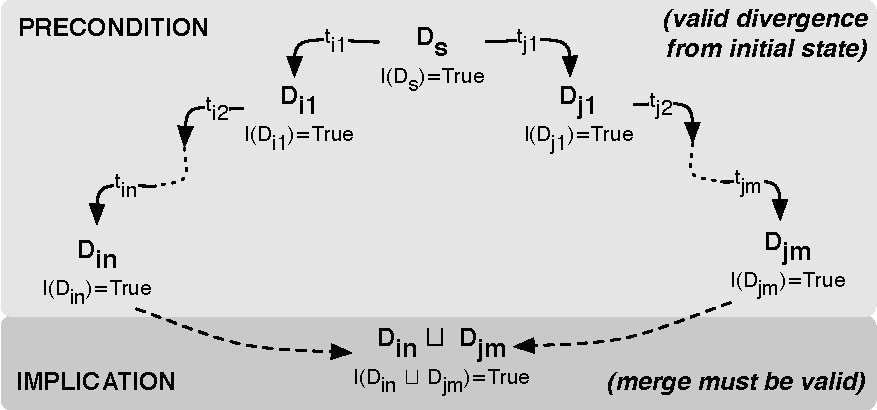
\includegraphics[width=\columnwidth]{figs/icommute.pdf}\vspace{-1em}
\end{center}
\caption{An \iconfluent execution illustrated via a diamond
  diagram. If a set of transactions $T$ is \iconfluent, then all
  database states reachable by executing and merging transactions in
  $T$ starting with a common ancestor ($D_s$) must
  be mergeable ($\sqcup$) into an $I$-valid database state.}
\label{fig:iconfluence}
\end{figure}

\subsection{\iconfluence and Coordination}
\label{sec:ic-result}

We can now apply \iconfluence to our goals from Section~\ref{sec:model}:

\begin{theorem}
\label{theorem:necessary}
A globally $I$-valid system can execute a set of transactions $T$ with
\cfreedom, transactional availability, convergence if and only if $T$
is \iconfluent with respect to $I$.
\end{theorem}

We provide a full proof of Theorem~\ref{theorem:necessary}
in~\rappendix{\apptheory} (which is straightforward) but provide a
sketch here. The backwards direction is by construction: if
\iconfluence holds, each replica can check each transaction's
modifications locally and replicas can merge independent modifications
to guarantee convergence to a valid state. The forwards direction uses
a partitioning argument~\cite{gilbert-cap} to derive a contradiction:
we construct a scenario under which a system cannot determine whether
a non-\iconfluent transaction should commit without violating one of
our desired properties (either compromising validity or availability,
diverging forever, or coordinating).

Theorem~\ref{theorem:necessary} establishes \iconfluence as a
necessary and sufficient condition for invariant-preserving,
coordination-free execution.  If \iconfluence holds, there exists a
correct, coordination-free execution strategy for the transactions; if
not, no possible implementation can guarantee these properties for the
provided invariants and transactions. That is, if \iconfluence does
not hold, there exists at least one execution of transactions on
separate replicas that will violate the given invariants when servers
converge. To prevent invalid states from occurring, at least one of
the transaction sequences will have to forego availability or
\cfreedom, or the system will have to forego convergence. \iconfluence
analysis is independent of any given implementation, and effectively
``lifts'' prior discussions of scalability, availability, and low
latency~\cite{hat-vldb,gilbert-cap,pacelc} to the level of application
(i.e., not ``I/O''~\cite{consistency-borders}) correctness. This
provides a useful handle on the implications of coordination-free
execution without requiring reasoning about low-level properties such
as physical data location and the number of servers.

\subsection{Discussion and Limitations}
\label{sec:theory-discussion}

\iconfluence captures a simple (informal) rule:
\textbf{\textit{coordination can only be avoided if all local commit
    decisions are globally valid}}. (Alternatively, commit decisions
are composable.) If two independent decisions to commit can result in
invalid converged state, then replicas must coordinate in order to
ensure that only one of the decisions is to commit. Given the
existence of an unsafe execution and the inability to distinguish
between safe and invalid executions using only local information, a
globally valid system \textit{must} coordinate in order to prevent the
invalid execution from arising.

\minihead{Use of invariants} Our use of invariants in \iconfluence is
key to achieving a \textit{necessary} and not simply sufficient
condition. By directly capturing application-level correctness
criteria via invariants, \iconfluence analysis only identifies
``true'' conflicts. This allows \iconfluence analysis to perform a
more accurate assessment of whether coordination is needed compared to
related conditions such as commutativity
(Section~\ref{sec:relatedwork}).

However, the reliance on invariants also has drawbacks. \iconfluence
analysis only guards against violations of any provided invariants. If
invariants are incorrectly or incompletely specified, an \iconfluent
database system may violate application-level correctness. If users
cannot guarantee the correctness and completeness of their invariants
and operations,
they should opt for a more conservative analysis or mechanism such as
employing serializable transactions. Accordingly, our development of
\iconfluence analysis provides developers with a powerful option---but
only if used correctly. If used incorrectly, \iconfluence allows
incorrect results, or, if not used at all, developers must resort to existing alternatives.

This final point raises several questions: can we specify invariants
in real-world use cases? Classic database concurrency control models
assume that ``the [set of application invariants] is generally not
known to the system but is embodied in the structure of the
transaction''~\cite{traiger-tods,eswaran-consistency}. Nevertheless,
since 1976, databases have introduced support for a finite set of
invariants~\cite{korth-serializability,decomp-semantics,garciamolina-semantics,ic-survey,ic-survey-two}
in the form of primary key, foreign key, uniqueness, and row-level
``check'' constraints~\cite{kemme-si-ic}. We can (and, in this paper,
do) analyze these invariants, which can---like many program
analyses~\cite{kohler-commutativity}---lead to new insights about
execution strategies. We have found the process of invariant
specification to be non-trivial but feasible in practice;
Section~\ref{sec:evaluation} describes some of our experiences.

\minihead{(Non-)determinism} \iconfluence analysis effectively
captures points of \textit{unsafe
  non-determinism}~\cite{consistency-borders} in transaction
execution. As we have seen in many of our examples thus far, total
non-determinism under concurrent execution can compromise
application-level consistency~\cite{calm,termrewriting}. But not all
non-determinism is bad: many desirable properties (e.g.,
classical distributed consensus among processes) involve forms 
of acceptable non-determinism (e.g., any proposed outcome is
acceptable as long as all processes agree)~\cite{paxos-commit}. In
many cases, maximizing safe concurrency requires non-determinism.

\iconfluence analysis allows this non-deterministic divergence of
database states but makes two useful guarantees about those
states. First, the requirement for global validity ensures safety (in
the form of invariants). Second, the requirement for convergence
ensures liveness (in the form of convergence). Accordingly, via its
use of invariants, \iconfluence allows users to scope non-determinism
while permitting only those states that are acceptable.



